\documentclass[11pt]{article}
\usepackage{natbib}
\usepackage{fullpage}
\usepackage{fancyhdr}

\usepackage{amsmath}
\usepackage{amssymb}
\usepackage{url}

\usepackage{listings}
\usepackage{color}
\lstset{language=Python,
        basicstyle=\footnotesize\ttfamily,
        showspaces=false,
        showstringspaces=false,
        tabsize=2,
        breaklines=false,
        breakatwhitespace=true,
        identifierstyle=\ttfamily,
        keywordstyle=\color[rgb]{0,0,1},
        commentstyle=\color[rgb]{0.133,0.545,0.133},
        stringstyle=\color[rgb]{0.627,0.126,0.941},
    }

\usepackage{graphicx}

% header
\fancyhead{}
\fancyfoot{}
\fancyfoot[C]{\thepage}
\fancyhead[R]{Daniel Foreman-Mackey}
\fancyhead[L]{Statistical Natural Language Processing --- Homework 3}
\pagestyle{fancy}
\setlength{\headsep}{10pt}
\setlength{\headheight}{20pt}

% shortcuts
\newcommand{\Eq}[1]{Equation (\ref{eq:#1})}
\newcommand{\eq}[1]{Equation (\ref{eq:#1})}
\newcommand{\eqlabel}[1]{\label{eq:#1}}
\newcommand{\Fig}[1]{Figure~\ref{fig:#1}}
\newcommand{\fig}[1]{Figure~\ref{fig:#1}}
\newcommand{\figlabel}[1]{\label{fig:#1}}

\newcommand{\pr}[1]{\ensuremath{p\left (#1 \right )}}
\newcommand{\lk}[1]{\ensuremath{\mathcal{L} \left ( #1 \right )}}
\newcommand{\bvec}[1]{\ensuremath{\boldsymbol{#1}}}
\newcommand{\dd}{\ensuremath{\, \mathrm{d}}}
\newcommand{\normal}[2]{\ensuremath{\mathcal{N} \left ( #1; #2 \right ) }}
\newcommand{\T}{^\mathrm{T}}

\newcommand{\data}{\mathcal{D}}
\newcommand{\code}[1]{{\sffamily #1}}


\begin{document}

As with the last assignment, I decided to implement my homework in Python
instead of using the provided Java code.
I was surprised to find that the language modeling implemented in pure-Python
was very computationally efficient.
This is because the data structures in the standard library are pretty
impressive!
I also started implementing a version that looked a bit more like the provided
code (using a lot of objects) and that was painfully slow.
I wasn't able to make the Viterbi algorithm bearable in pure-Python so I
dropped down to C for that part (but I still evaluate the trigram/emission
model using Python).
All of the code that I used for this assignment is available on GitHub:
\url{https://github.com/dfm/nlp}.

\section{The Model}

The problem that we're trying to solve in this assignment is: given a
sentence $\bvec{w} = \{w_1, w_2, \ldots, w_n\}$, what is the part of
speech $t_i$ associated with each word $w_i$.
The model that we're considering is the simple hidden Markov model (HMM) shown
in \fig{pgm}\footnote{This graphical model figure was generated using my
Python module called Daft \url{http://daft-pgm.org} $<$/advertisement$>$}.
This model relies on two generative probability distributions
\begin{eqnarray}
& p(t_i \,|\, t_{i-2},\,t_{i-1}) & \quad \mathrm{transitions} \\
& p(w_i \,|\, t_i) & \quad \mathrm{emissions}
\end{eqnarray}
These are the relevant quantities because we are looking to find the tag
sequence $\bvec{t}$ that maximizes the posterior probability distribution
\begin{eqnarray}
p(\bvec{t}\,|\,\bvec{w}) &=& \frac{p(\bvec{t},\,\bvec{w})}{p(\bvec{w})}
                             \nonumber\\
                         &\propto& p(\bvec{t},\,\bvec{w}) \nonumber\\
                         &=& \prod_i p(t_i \,|\, t_{i-2},\,t_{i-1}) \,
                                     p(w_i \,|\, t_i) \quad.
\end{eqnarray}
The following sections describe the different methods for estimating these
distributions and the results of more sophisticated models.

\begin{figure}[htbp]
\begin{center}
    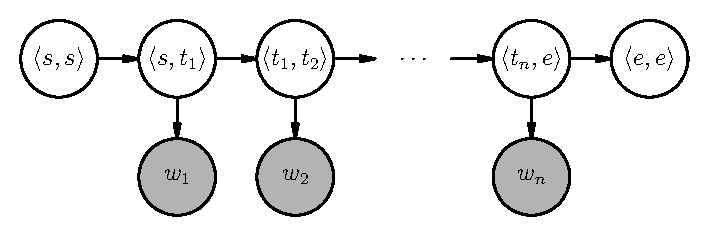
\includegraphics{pgm.pdf}
\end{center}
\caption{%
\figlabel{pgm}}
\end{figure}

\section{The Baseline Model}

The first model that I built was similar to the \emph{Baseline} model in the
provided code but with a slightly different model of unknown word
probabilities (with similar performance).
In this model, the tag context is ignored and instead, the tag probabilities
are given by the function (estimated from the training data)
\begin{eqnarray}\eqlabel{cond-emission}
p(t_i\,|\,w_i) &=& \frac{f(t_i,w_i)}{f(w_i)}
\end{eqnarray}
where $f(t_i, w_i)$ is a count of the number of times the word $w_i$ appears
with the part-of-speech tag $t_i$ in the training set.
Similarly, $f(w_i)$ is the total number of times the word $w_i$ appears in the
training examples.
This simple model clearly breaks down for words that have never been seen
giving exactly zero probability to each tag.

\paragraph{Unknown words}
The provided code deals with this by building a second distribution
\begin{eqnarray}
p(t_i\,|\,\mathrm{unk})
\end{eqnarray}
that is estimated from the training data by looping through the training data
and counting the number of times the tag $t_k$ is associated with the
\emph{first appearance} of the word $w_n$.
This seems like a reasonable model but for consistency with my better unknown
word model, I made a simpler model
\begin{eqnarray}
p(t_i\,|\,\mathrm{unk}) &=& \frac{\left . f(t_i)\right |_\theta}{N_\theta}
\end{eqnarray}
where $\left.f(t_i)\right|_\theta$ is the number of times the tag $t_i$
appears in a subset of the training data $\theta$ and $N_\theta$ is the number
of examples in the same subset.
I chose the ``unknown proxy'' subset by counting the number of times each word
appears in the full training corpus and extracting all the examples that emit
words that appear fewer than $K$ times.
This adds a free parameter to the model but I found that the performance
wasn't particularly sensitive to the choice for $1 \lesssim K \lesssim 10$
(I'll come back to this later in mode detail).
This model does seem to do surprisingly well but there's a lot we can do to
make it better.

\section{Trigram Transitions}

The first step in building a better model is to take the local context into
account.
In particular, we'll consider condition on the two previous tags to compute
the transition probabilities.
Following \citet{tnt}, I estimated the transition probabilities using the
linearly interpolated form
\begin{eqnarray}\eqlabel{trigram}
p(t_i\,|\, t_{i-2},\,t_{i-1}) & = &
    (1-\lambda_2-\lambda_3)\,\hat{p}(t_i) +
    \lambda_2\,\hat{p}(t_i\,|\,t_{i-1}) +
    \lambda_3\,\hat{p}(t_i\,|\,t_{i-2},\,t_{i-1})
\end{eqnarray}
where
\begin{eqnarray}
\hat{p}(t_i) &=& \frac{f(t_i)}{N} \\
\hat{p}(t_i\,|\,t_{i-1}) &=& \frac{f(t_{i-1},t_i)}{f(t_{i-1})} \\
\hat{p}(t_i\,|\,t_{i-2},\,t_{i-1}) &=&
    \frac{f(t_{i-2},t_{i-1},t_i)}{f(t_{i-2},t_{i-1})}
\end{eqnarray}
and $N$ is the total number of tag trigrams in the training set and $f(\cdot)$
is the count of the number of times the given tag sequence is observed in
the training data.
This model adds two more free parameters that need to be chosen properly.
My preferred method would be to determine these values using cross-validation
but given the large computational cost, I instead implemented the deleted
interpolation method as described by \citet{tnt}.
Using this method, I estimated the optimal parameters to be:
\begin{eqnarray}
    \lambda_2 &=& 0.2778 \quad \mathrm{and} \nonumber\\
    \lambda_3 &=& 0.5709 \quad.
\end{eqnarray}
In practice, I found that the rounded values $\lambda_2 = 0.3$ and
$\lambda_3 = 0.6$ gave marginally better performance on both the in-domain
and out-of-domain validation sets so I'll stick to that for the rest of this
write-up.

\section{A Better Model of Emission Probabilities}

For my model of the emission probability distribution $p(w_i\,|\,t_i)$, I
again inferred an empirical distribution based directly on the frequencies in
the training set.
As a result, I estimated this distribution as
\begin{eqnarray}\eqlabel{emission}
p(w_i\,|\,t_i) = \frac{f(t_i,w_i)}{f(t_i)}\quad.
\end{eqnarray}
This is similar to \eq{cond-emission} but instead of estimating the tag
probabilities conditional on the observed word, I directly estimated the
likelihood function.

\section{Unknown Words Revisited}

The model in \eq{emission} will still give a model with any new words a
probability of exactly zero so this is clearly not acceptable.
To deal with this, I also built a more sophisticated feature-based unknown
word model.
The model that I settled on was a very simple---fast to train and
evaluate---empirical model based on a set of engineered features.
I expect that a probabilistic discriminative classifier like the Maximum
Entropy model that we implemented in the previous assignment would offer
somewhat better performance at the cost of a much more computationally
expensive training period.
My empirical model trains quickly with a single pass through the training data
and the evaluation cost also somewhat lower than the MaxEnt model.
Despite all this, the performance on unknown words is (as you will see below)
very competitive after a bit of tuning.

The features that I chose to use are:
\begin{itemize}
\item{a smoothed suffix distribution,}
\item{the case of the first character, and}
\item{an indication of the existence of numbers in the word.}
\end{itemize}

The smoothed suffix distribution looks similar to \eq{trigram} above but for
the final $N$ characters of the word.
I chose to use up to 3 letters because this keeps the model relatively small
while still offering a lot of flexibility.
In this case, the estimate of the unknown word suffix probability
distribution (to be trained on the subset of the training data discussed
above) is the following
\begin{eqnarray}\eqlabel{psuff}
p_\mathrm{suff}(w_i\,|\,t_i) &=& \theta_0\frac{f(t_i)}{N_\theta} +
    \frac{\theta_1\,f(t_i,\,\mathrm{suff}_1[w_i])
          + \theta_2\,f(t_i,\,\mathrm{suff}_2[w_i])
          + \theta_3\,f(t_i,\,\mathrm{suff}_3[w_i])}{f(t_i)}
\end{eqnarray}
where $\theta_0 = 1 - \theta_1 - \theta_2 - \theta_3$ and
$\mathrm{suff}_m[w_i]$ indicates the last $m$ letters of the word $w_i$.

I also built an empirical probability distribution for capitalization
conditioned on the tags based on the same training subset.
\begin{eqnarray}\eqlabel{pcap}
p_\mathrm{cap} (w_i\,|\,t_i) &=&
    \frac{f(t_i,\,\mathrm{cap}[w_i])+1}{N_\theta+1}
\end{eqnarray}
where the $\mathrm{cap}$ function is defined as
\begin{eqnarray}
\mathrm{cap}(w_i) &=& \left \{ \begin{array}{ll}
    0 & \mbox{if the first letter of $w_i$ is lowercase,} \\
    1 & \mbox{if the first letter of $w_i$ is uppercase.} \\
\end{array}\right .
\end{eqnarray}
The added one in \eq{pcap} is there as a smoothing term to make sure that this
probability never goes to exactly zero.

The final feature of my unknown word model is a count of the number of digits
in the word.
I tried just using a flag indicating the existence of (at least) one number in
the word but I found that a richer structure provided a somewhat better
out-of-domain validation set performance.
In the end, the best results that I found resulted from a model that I built
by estimating a probability of observing a word with $K$ digits for each tag
\begin{eqnarray}\eqlabel{pnum}
p_\mathrm{num}(w_i\,|\,t_i) &=&
    \frac{f(t_i,\,\mathrm{digits}[w_i])+1}{f(t_i)+K}
\end{eqnarray}
where
\begin{eqnarray}
\mathrm{digits}[w_i] &=& \left \{ \begin{array}{ll}
    0 & \mbox{if there are no digits in $w_i$,} \\
    1 & \mbox{if there is one digit in $w_i$,} \\
    \cdots & \\
    K & \mbox{if there are $\ge K$ digits in $w_i$.}
\end{array}\right.
\end{eqnarray}
Note that \eq{pnum} is smoothed in the same way as \eq{pcap}.

Combining the above features, we get the full probability distribution for
unknown words
\begin{eqnarray}\eqlabel{pfull}
p(w_i\,|\,t_i) &=& p_\mathrm{suff}(w_i\,|\,t_i) \,
                   p_\mathrm{cap}(w_i\,|\,t_i) \,
                   p_\mathrm{num}(w_i\,|\,t_i) \quad.
\end{eqnarray}
Because of the smoothing applied to each term in this product, this
probability should never be exactly zero.
This is necessary because the features are not a perfect set of summary
statistics and in practice some validation examples end up getting zero
probability for \emph{every tag sequence}.
This would make inference impossible and it is clearly an artificial effect
since we are explicitly discussing \emph{unknown words}.

\paragraph{Rejected features}
I considered various other features that I ended up rejecting because they
made no effect on the validation performance (or sometimes even made the
results worse).
One feature that I considered was the existence of \emph{punctuation} in the
word.
My expectation was that unrecognized punctuation would be better classified by
including this feature.
Instead, most punctuation errors seem to be related to differences between the
``gold'' tag rules of the in-domain and out-of-domain datasets.
I'll discuss this fact in more depth below.

\section{Inference}

The previous sections describe the form of the probabilistic generative model
that we'll assume for this problem.
They also explain the training procedure given a set of tagged sentences.
Given this trained model, the only step left is inference: finding the tag
sequence that maximizes the posterior probability.
The baseline model in the provided code implements a greedy inference
procedure.
This is a very computationally efficient technique because it only requires a
single pass through the sentence and at each word, it only requires the
evaluation of a single set of conditional probabilities.
The problem is that it doesn't have any guarantee of finding the true maximum
probability path.

\paragraph{Viterbi algorithm}
For the HMM model described by \fig{pgm}, it is possible---and relatively
efficient---to compute the exact maximum \emph{a posteriori} path using the
Viterbi method.
Qualitatively, this method works by iterating through the words in the
sentence and at each word $w_i$, evaluating and saving---for each tag
$t_i$---the preceding path of tags $\bvec{t}_{<i}$ that gives the maximum
probability up to the word $i$.
It's easy to see that by the time you've iterated through the entire sentence,
the maximum probability tag will exactly define the best path.
This method is no longer exponential---like the na\"ive method---but it is
still relatively computationally expensive.
One optimization that I implemented is to explicitly exclude any zero
probability paths so that you don't have to compute the probabilities
conditioned on those paths.
In this case, this helps \emph{a lot} because many words cannot possibly be
generated by a given tag.
Another optimization that would probably be very useful in a real world
application---but I didn't implement it this time---would be to prune the tree
with some relative probability threshold at each step.
In other words, exclude any tags that give a probability less than some
$\theta < 1$ times the maximum probability at that step.
This would be similar to a beam search algorithm but I expect that it would be
more reliable because at uncertain steps---where each possible branch has
close to the same probability---many of the branches would be thrown away by a
beam search whereas this pruned Viterbi method would keep more possibilities
open.

\section{Results}

In the previous section, I developed 4 different ``models'' for the
part-of-speech tagging problem:
\begin{enumerate}
\item{{\bf Baseline}: a context independent scorer using the greedy
      decoder,}
\item{{\bf Trigram}: a trigram scorer using the greedy decoder,}
\item{{\bf Viterbi}: the same trigram scorer using the exact Viterbi decoder,
      and}
\item{{\bf Unknown}: the same trigram scorer with a better model of unknown
      words using the Viterbi decoder.}
\end{enumerate}
The \emph{Baseline} model has one free parameter: the threshold count for
estimating the unknown word distribution.
The \emph{Trigram} and \emph{Viterbi} models have 2 extra parameters: the
$\lambda$ interpolation coefficients used by the trigram scorer.
My specific formulation of the \emph{Unknown} model adds 3 more parameters:
the $\theta$s controlling the interpolation in the suffix model.
Here, I will discuss the effects of each of these parameters on the in-domain
and out-of-domain validation sets.
In general, I found that the performance of all of my methods was
substantially ($\lesssim 2\%$) worse on the test data than on the
out-of-domain validation set but I was still able to achieve competitive
performance on all of the non-training data.

\subsection{The \emph{Baseline} model}

\section{Discussion}

\begin{thebibliography}{}\raggedright

\bibitem[Brants(2000)]{tnt} Thorsten Brants (2000)
\textbf{TnT---A Statistical Part-of-Speech Tagger}.
In \emph{Proceedings of the Sixth Applied Natural Language Processing
Conference}. Seattle, WA.

\end{thebibliography}

\end{document}
